\section{Scene analysis and synthesis}
\label{sec:scene}
% motivation
Analyzing and modeling indoor and outdoor environments has important applications in various domains. For example, in robotics it is desirable for an autonomous agent to understand the semantics of 3D environments to be able to interact with them. In urban planning and architecture, professionals build digital models of cities and buildings to validate and improve their designs. In computer graphics, artists create novel 3D scenes for movies and video games.


%\teaser{
\begin{figure}[t]
\centering
    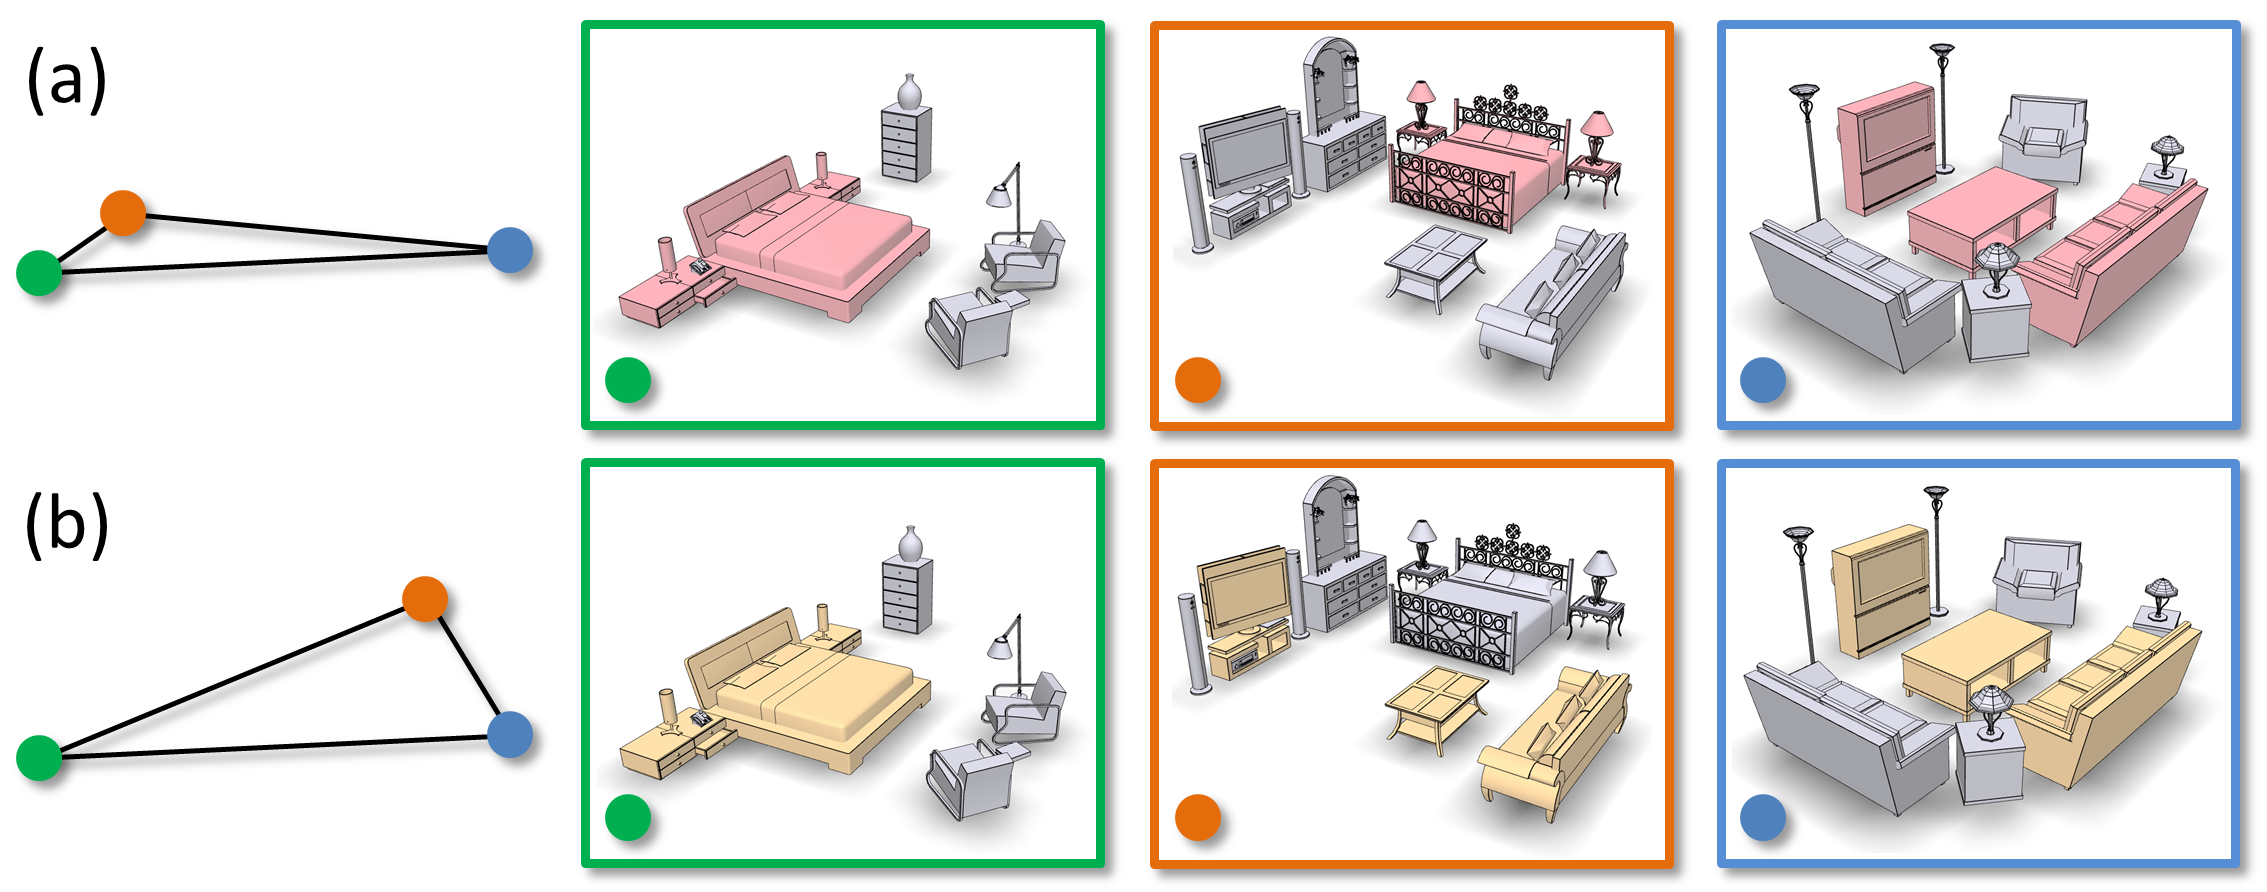
\includegraphics[width=0.99\linewidth]{fig/img/xu_sig14_focal}
    %\vspace{-0.2cm}
    \caption{
    Scene comparisons may yield different similarity distances (left) depending on the focal points~\cite{Xu:2014:OHSC}.}
    \label{fig:xu_sig14_focal}
\end{figure}
%}


% opportunities and challenges
The fast growing number of 3D scenes in digital repositories provide new opportunities for data-driven scene analysis, editing, and synthesis. Emerging collections of 3D scenes pose novel research challenges that cannot be easily addressed with existing tools.  In particular, representations created for analyzing collections of single models mostly focus on arrangement and relations between shape parts~\cite{Mitra:2014:SASP}, which usually exhibit less variations than objects in scenes. Capturing scene structure poses a greater challenge due to looser spatial relations and a more diverse mixture of functional substructures.

%
%The analysis of model collections has been prevalently focused on single objects.
%where the main focus of study is the arrangement and relations between shape parts, and their connection with functionality or semantics~\cite{Mitra:2014:SASP}.
%Compared to the structure of shape parts in a single object, the structural layout of objects in a scene is more complex due to the looser spatial relations and a more diverse mixture of functional substructures.

% previous work on image understanding
Inferring scene semantics is a long-standing problem in image understanding, with many methods developed for object recognition~\cite{quattoni2009}, classification~\cite{swadzba2010},
layout and structure reasoning~\cite{Choi:2013:UIS,Fouhey:2013:DDP} with \emph{a single image}. Previous work demonstrates that one can leverage collections of 3D models to facilitate scene understanding in images~\cite{Satkin:2012:DDS}.
In addition, the depth information in RGBD scans can be used to establish the link between 2D and 3D for model-driven scene understanding~\cite{Silberman:2012:ISS}. The semantic annotations of images are not immediately useful for modeling and synthesizing 3D scenes, for which the geometric and structural priors have to be learned from 3D data.

In this section, we cover the data-driven techniques that leverage collections of 3D scenes for modeling, editing, and synthesizing novel scenes.

%In this section, we will mainly cover works on scene analysis and synthesis
%from the graphics community, with the main focus on 3D indoor scenes.

\paragraph*{Context-based retrieval.}
To address the large variation in the geometry and arrangement of objects in scenes, Fisher et al.~\cite{Fisher:2010:CSM,Fisher:2011:CSR} propose to take advantage of local context.  One of the key insights of their work is that collections of 3D scenes provide rich information about context in which objects appear. They show that capturing these contextual priors can help in scene retrieval and editing.

Their system takes an annotated collection of 3D scenes as input, where each object in a scene is classified. They represent each scene as a graph, where nodes represent objects and edges represent relations between objects, such as support and surface contact. In order to compare scenes, they define kernel functions for pairs of nodes measuring similarity in object geometry, and for pairs of edges, measuring similarity in relations of two pairs of objects.  They further define a graph kernel to compare pairs of scenes.  In particular, they compare all walks of fixed length originating at all pairs of objects in both scene graphs, which loosely captures similarities of all contexts in which objects appear~\cite{Fisher:2011:CSR}.  They show that this similarity metric can be used to retrieve scenes. By comparing only paths originated at a particular object, they can retrieve objects for interactive scene editing.

%Their scene editing interface also allows retrieving relevant models by placing bounding boxes into partially modeled scenes, where the system returns a most relevant object that conforms to box dimensions and contextual relationship to the surrounding objects~\cite{Fisher:2010:CSM}.


%model spatial relationship between pairs of objects using kernel density estimation~\cite{Fisher:2010:CSM}. Such learned spatial relationship can be used in context-based object retrieval, which can be quite effective in assisting interactive scene modeling. For example, the user places a bounding box into the partially modeled scene as a proxy and the system can return a relevant object which both conforms to the size of the proxy and admits the contextual relationship against the surrounding objects.
%
%Later, Fisher et al. propose the first similarity measure for 3D scenes through
%representing scenes as graphs which encode models and their contextual relationships and then
%defining a kernel between the relationship graphs~\cite{Fisher:2011:CSR}.
%Such graph kernel based scene similarity is shown to be discriminative for scene retrieval.
%Meanwhile, since the graph kernel integrates spatial relationships between all objects in the scene,
%it is also informative in characterizing contextual information and outperforms their previous method~\cite{Fisher:2010:CSM}
%for context-based object retrieval.



\paragraph*{Focal points.}
Measuring the similarity of complex hybrid scenes such as studios composed of a bedroom, living room, and dining room poses a challenge to graph kernel techniques since they only measure global scene similarity. Thus, Xu et al.~\shortcite{Xu:2014:OHSC} advocate analyzing salient sub-scenes, which they call focal points, to compare hybrid scenes, i.e., scenes containing multiple salient sub-scenes. Figure~\ref{fig:xu_sig14_focal} shows an example of comparing complex scenes, where
the middle scene is a hybrid one encompassing two semantically salient sub-scenes, i.e., bed-nightstands and TV-table-sofa.
The middle scene is closer to the left one when the bed and nightstands are focused on, and otherwise when the TV-table-sofa combo is the focal point.
Therefore, scene comparison may yield different similarity distances depending on the focal points.

Formally, a focal point is defined as a representative substructure of a scene which can characterize a semantic scene category. That means the substructure should re-occur frequently only within that category. Therefore, focal point detection is naturally coupled with the identification of scene categories via scene clustering. This poses coupled problems of detecting focal points based on scene groups and grouping scenes based on focal points.
These two problems are solved via interleaved optimization which alternates between focal point detection and focal-based scene clustering. The former is achieved by mining frequent substructures and the latter uses subspace clustering, where scene distances are defined in a focal-centric manner.  Inspired by the work of Fisher et al.~\cite{Fisher:2011:CSR}, scene distances are computed using focal-centric graph kernels which are estimated from walks originating from representative focal points.


\begin{figure}[t] \centering
    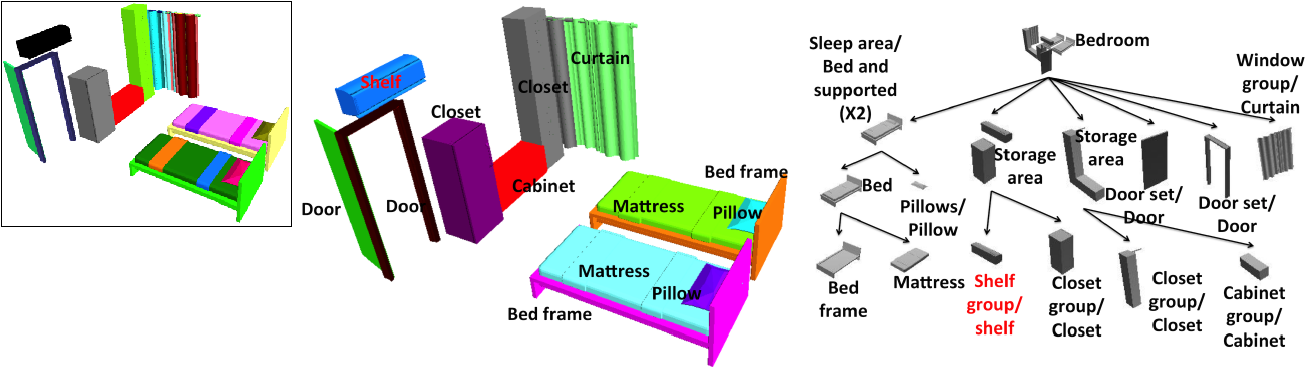
\includegraphics[width=0.98\linewidth]{fig/img/liu_siga14_sh}
        %\vspace{-0.3cm}
    \caption{
    The algorithm processes raw scene graphs with possible over-segmentation (a) into consistent hierarchies capturing semantic and functional groups (b,c)~\cite{Liu:2014:CCS}.
    }
    \label{fig:liu_siga14_sh}
\end{figure}


%
The detected focal points can be used to organize the scene collection and to support efficient exploration of the collection (see Section~\ref{sec:exploration}). Focal-based scene similarity can be used for novel applications such as multi-query scene retrieval,
where one may issue queries consisting of multiple semantically related scenes and wish to retrieve more scenes ``of the same kind''.% (Figure~\ref{fig:multiquery}).

%
\begin{figure}[t] \centering
    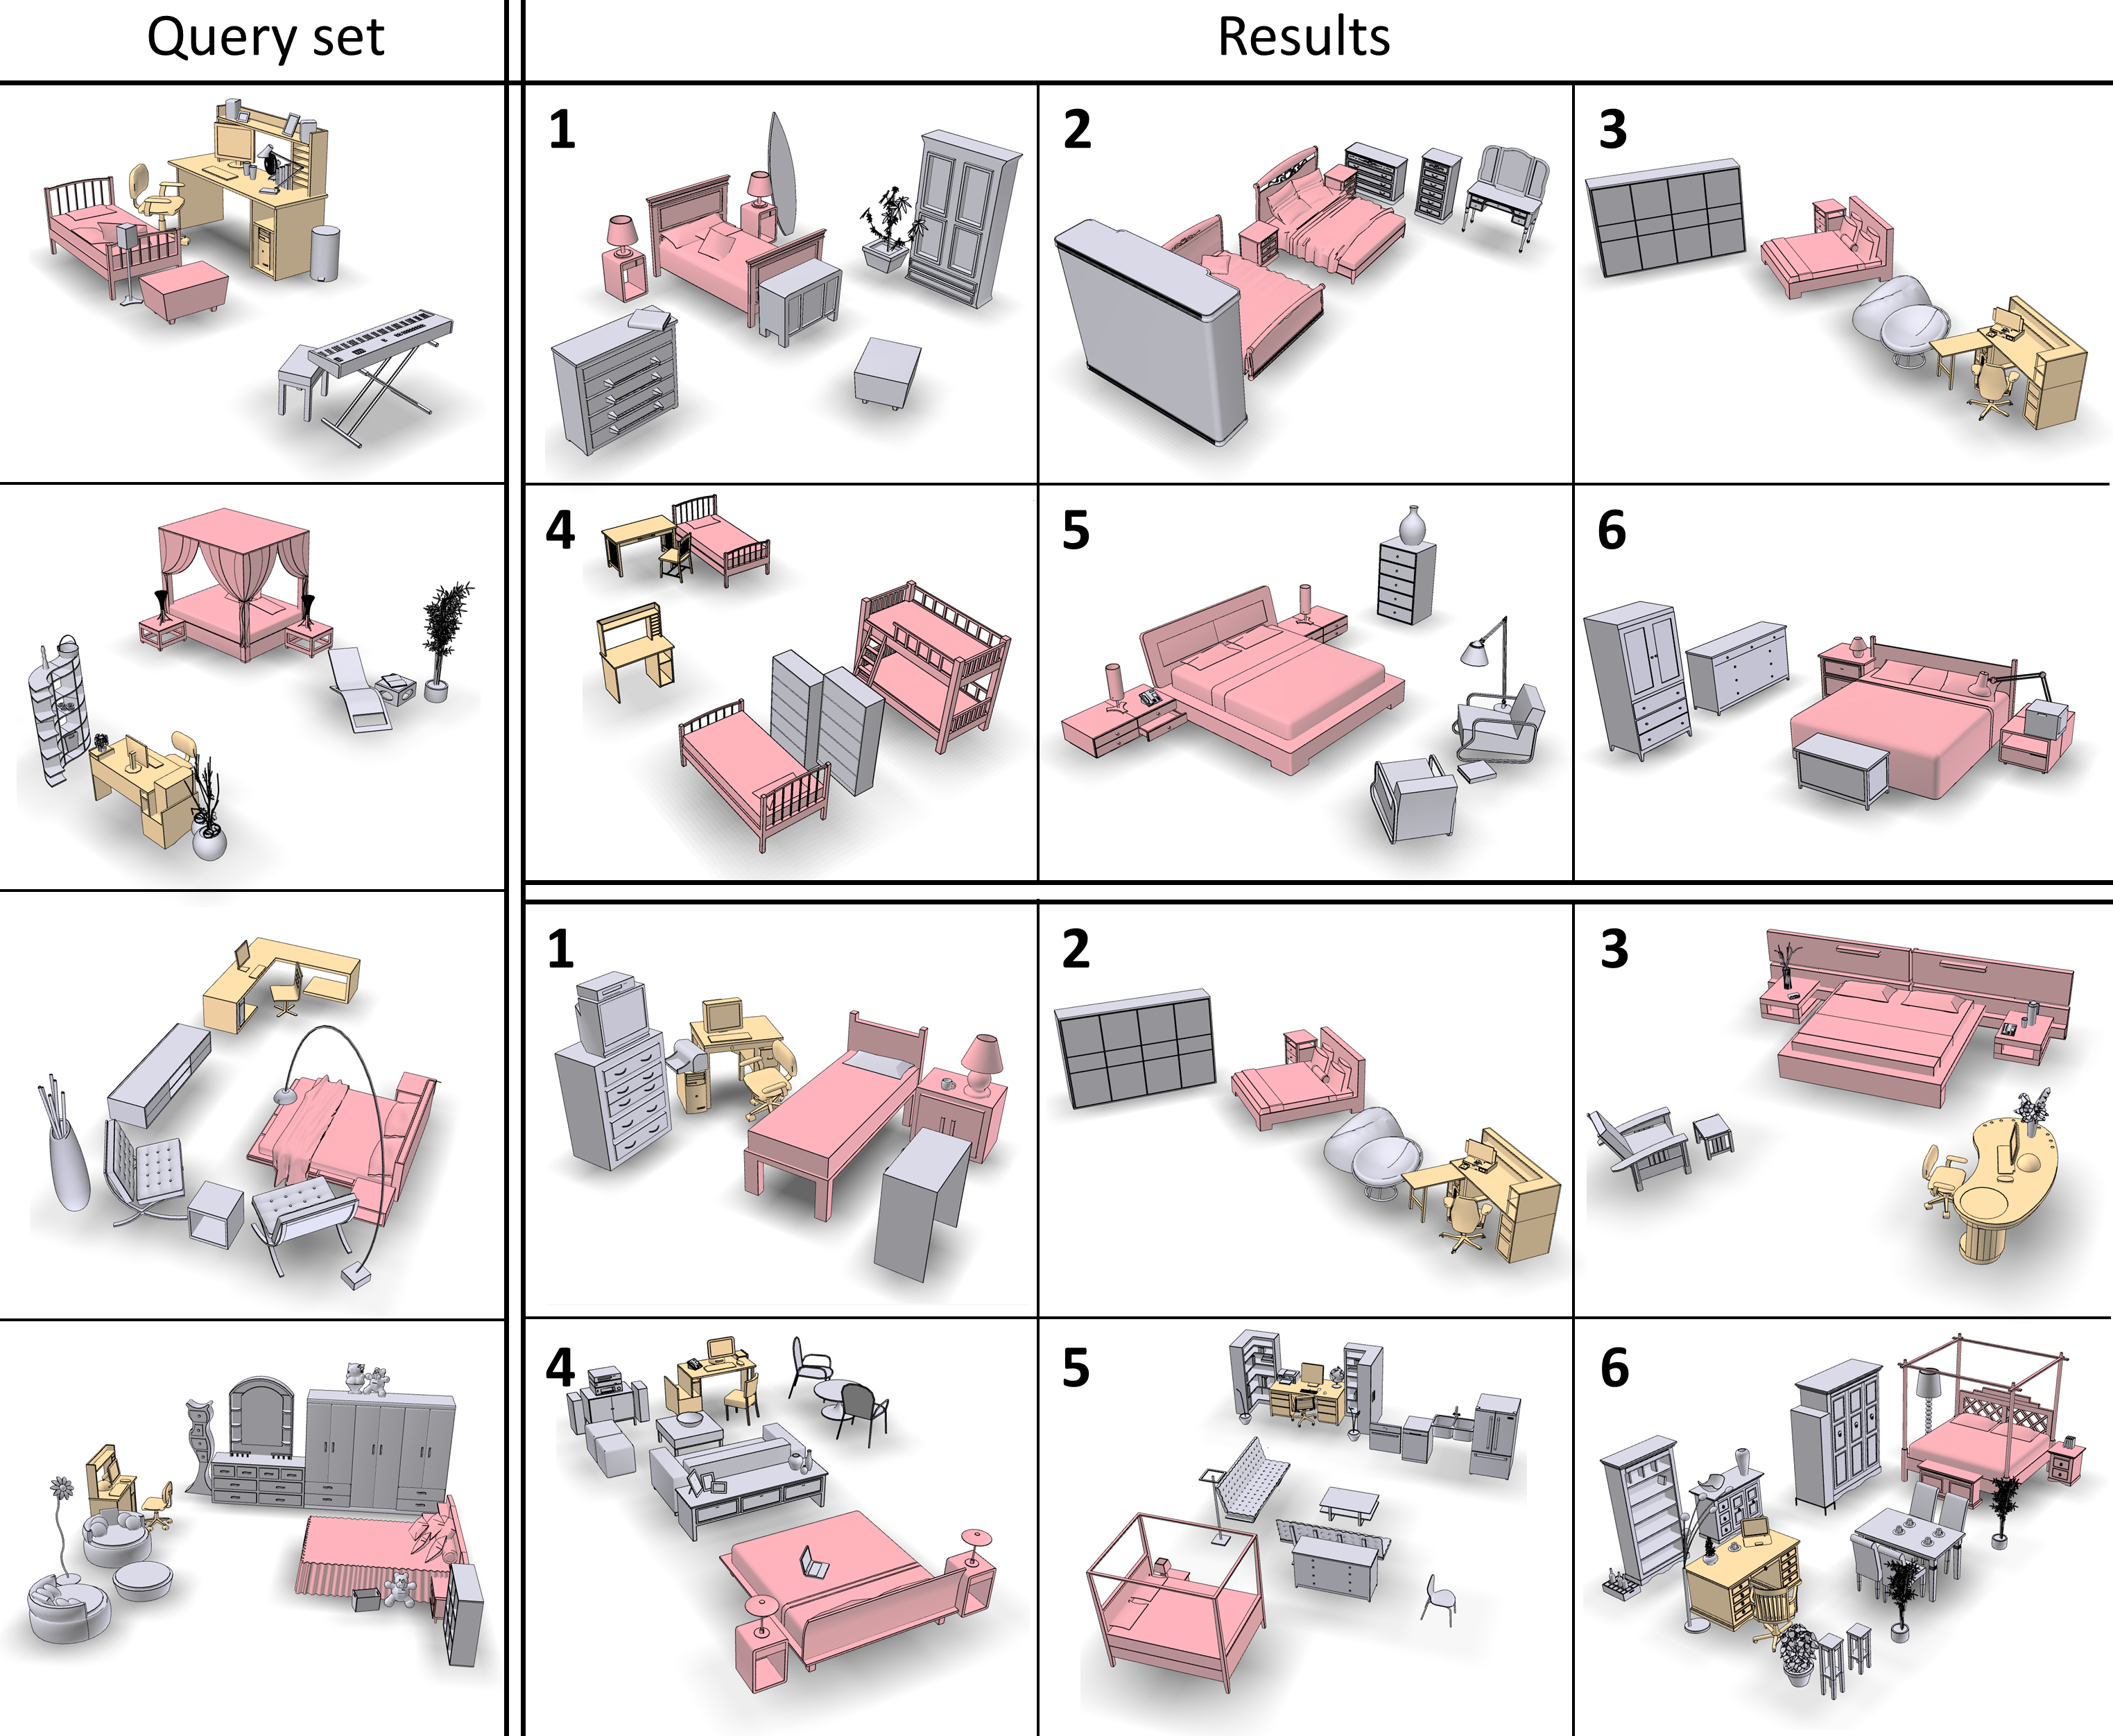
\includegraphics[width=0.98\linewidth]{fig/img/xu_sig14_multiquery}
        \vspace{-0.4cm}
    \caption{
    Multi-query retrieval takes a query set (left) and returns a ranked list of scenes (bottom-right) via focal (colored red and yellow) based scene comparison.
    Returns based on global scene similarity computed by graph kernel are also shown (top-right).
    }
    \vspace{-0.6cm}    
    \label{fig:multiquery}
\end{figure}


\paragraph*{Synthesis.}
Given an annotated scene collection, one can also synthesize new scenes that have a similar distribution of objects. The scene synthesis technique of Fisher et al.~\shortcite{Fisher:2012:CSR} learns two probabilistic models from the training dataset: (1) object occurrence, indicating which objects should be placed in the scene, and (2) layout optimization, indicating where to place the objects. Next, it takes an example scene, and then synthesizes similar scenes using the learned priors. It replaces or adds new objects using context-based retrieval techniques, and then optimizes for object placement based on learned object-to-object spatial relations.  Synthesizing example scenes might be a challenging task, thus Xu et al.~\shortcite{Xu:2013:S2S} propose modeling 3D indoor scenes from 2D sketches, by leveraging a database of 3D scenes. Their system jointly optimizes for sketch-guided co-retrieval and co-placement of all objects.


\begin{figure}[t] \centering
    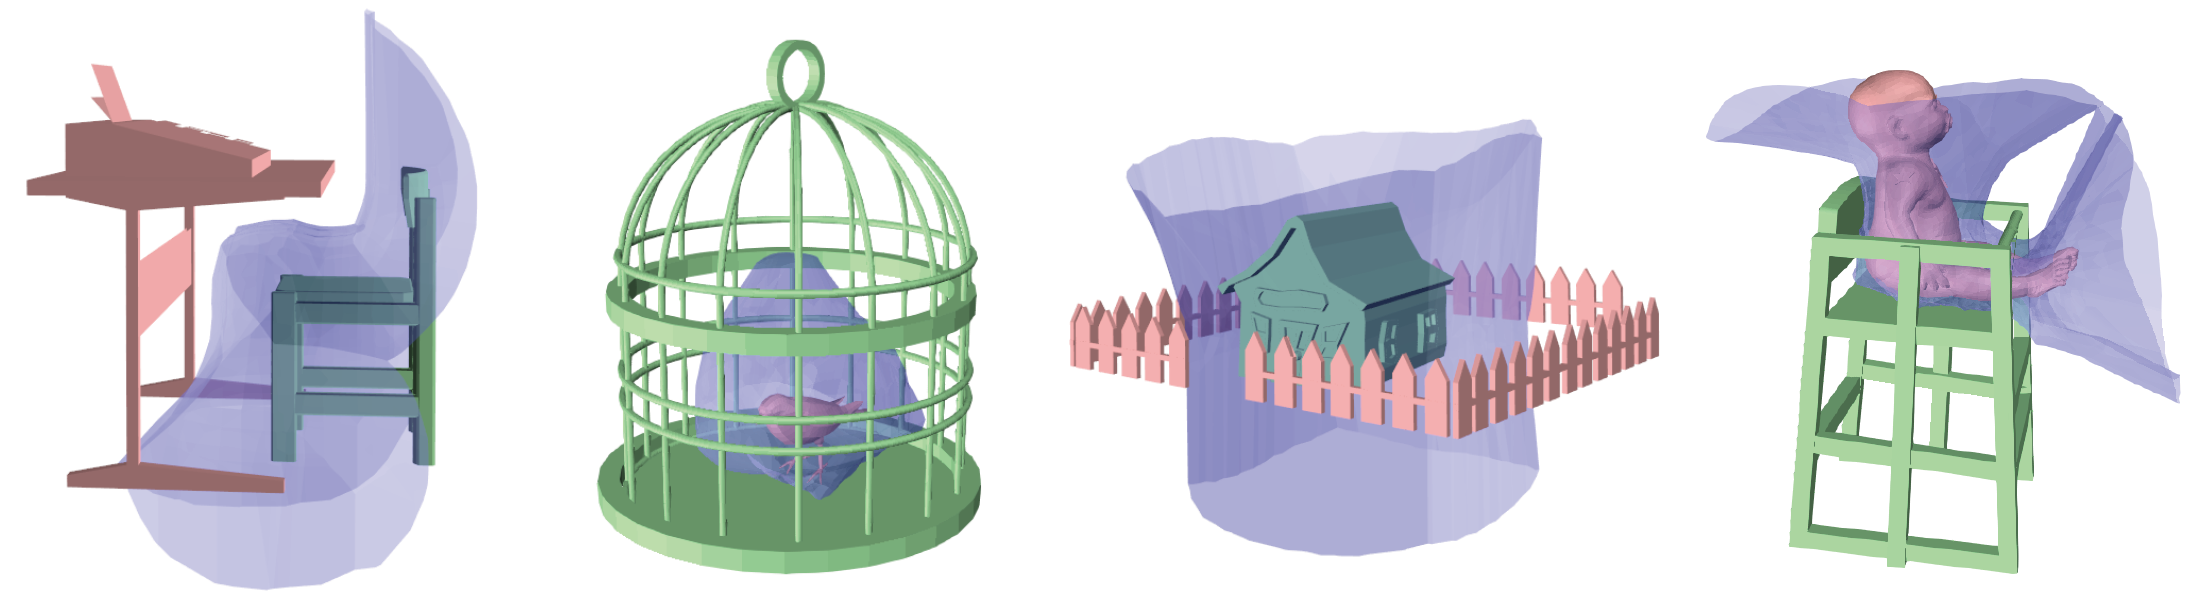
\includegraphics[width=0.99\linewidth]{fig/img/zhao_tog14_ibs}
    %\vspace{-0.2cm}
    \caption{
    The interaction bisector surface (in blue) of several two-object scenes~\cite{Zhao:2014:ISU}.
    }
    \label{fig:zhao_tog14_ibs}
\end{figure}


\paragraph*{Hierarchical scene annotation.}
All aforementioned applications take an annotated collection of 3D scenes as an input. Unfortunately, most scenes in public repositories are not annotated and thus require additional manual labeling~\cite{Fisher:2012:CSR}. Liu et al.~\shortcite{Liu:2014:CCS} address the challenge of annotating novel scenes. The key observation of their work is that understanding hierarchical structure of a scene enables efficient encoding of functional scene substructures, which significantly simplifies detecting objects and representing their relationships. Thus, they propose a supervised learning approach to estimate a hierarchical structure for novel scenes. Given a collection of scene graphs with consistent hierarchies and labels, they train a probabilistic hierarchical grammar encoding the distributions of shapes, cardinalities, and spatial relationships between objects. Such a grammar can then be used to parse new scenes: find segmentations, object labels, and hierarchical organization of objects consistent with the annotated collection (see Figure~\ref{fig:liu_siga14_sh}).

\paragraph*{Challenges and opportunities.}
The topic of 3D scene analysis is quite new and there are many open problems and research opportunities.
\emph{The first} problem is to efficiently characterize spatial relationships between objects and object groups. Most existing methods work with bounding box representation which are efficient to process, but not sufficiently informative to characterize object-to-object relationships.
For example, one cannot reliably determine the object enclosure relationship based on a bounding box.
Recently, He et al.~\shortcite{Zhao:2014:ISU} propose to use biologically-inspired bisector surface to characterize the
geometric interaction between adjacent objects and to index 3D scenes (Figure~\ref{fig:zhao_tog14_ibs}).
The bisector surface can be extended into a geometric descriptor for contextual modeling of the functionality of a 3D object in a given scene~\cite{hu:icon:2015}.
%
\emph{Second}, most existing techniques heavily rely on expert user supervision for scene understanding. Unfortunately, online repositories rarely have models with reliable object tags. Therefore there is a need for methods that can leverage scenes containing only partial and/or noisy annotations.
%most analysis rely on the availability of object labels, given the fact that the structural layout
%of scenes is mostly loose and spatial relationship is not always easy to be characterized geometrically.
%This is quite restrictive since most scene models from the web do not possess reliable object tag.
%Therefore, finding more powerful feature to characterize scenes and achieving tag-free analysis become indispensable.
%
\emph{Finally}, the popularity of commodity RGBD cameras has significantly simplified the acquisition of indoor scenes. This emerging scanning technique opens space for new applications such as online scene analysis~\cite{Zhang:2014:OSA,Xu:2015:ACS}.  %The availability of image data that come with RGBD scans also enables the enhancement of geometric representations with appearance information.

%On the other hand, the calibrated image and depth data help to relate 3D scenes with images, enabling bidirectional transfer of information such as labels, texture, etc.


